\documentclass[dvipdfmx]{jarticle}
\pagestyle{empty}
\usepackage{tikz}
\usetikzlibrary{shapes,calc}
\begin{document}
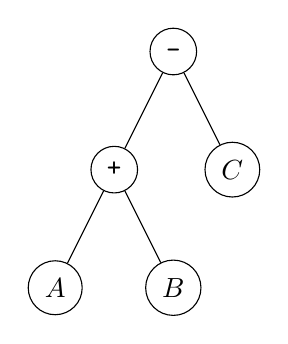
\begin{tikzpicture}
\node[draw,circle] (N1) at (0,0) {$A$};
\node[draw,circle] (N2) at (1.5,0) {$B$};
\node[draw,circle] (N3) at (0.75,1.5) {$\texttt{+}$};
\node[draw,circle] (N4) at (2.25,1.5) {$C$};
\node[draw,circle] (N5) at (1.5,3) {$\texttt{-}$};
\path[-] (N1) edge (N3) (N2) edge (N3) (N3) edge (N5) (N4) edge (N5);
\end{tikzpicture}
\end{document}